\chapter{الجهد الكيميائي والخلائط}\label{ch:b2:chemical-potential}

في الشتاء تنثر شاحنة الملح على طريق جليدي فيذوب الجليد عند
\qty{-10}{\celsius}؛ وسائل تبريد محرك السيارة، وهو ماء فيه ثلثه من
الإيثان-1,2-ديول، لا يتجمد في صقيع الليل ولا يغلي تحت غطاء محرك ساخن.
فالمادة المذابة تخفض درجة تجمد مذيبها وترفع درجة غليانه، وذلك، في
المحاليل المخففة، بمقدار يتعلق بعدد الجسيمات المذابة لا بطبيعتها. والأداة
التي تفسر ذلك هي \omterm{def:b2:chemical-potential:chemical-potential}{الجهد الكيميائي}، أي المشتقة الجزئية \omterm{def:b2:reaction-free-energy:gibbs-energy}{لطاقة جيبس} بالنسبة
إلى كمية مادة أحد المكوّنات. فهو يبيّن إلى أين «يريد أن يذهب» كل نوع
كيميائي، بين الأطوار وعبر التفاعلات، ويحوّل النشاطيات التي استعملها مجلد
السنة الأولى وصفاتٍ جاهزة إلى مقادير مشتقة.

\begin{recall}
\Cref{ch:b2:reaction-free-energy}: \omterm{def:b2:reaction-free-energy:gibbs-energy}{طاقة جيبس} $G = H - TS$، و$\dd G =
V\dd p - S\dd T + \Delta_r G\,\dd\xi$، ومحك التطور $\Delta_r G\,
\dd\xi \leq 0$. وكتب مجلد السنة الأولى نشاطية الغاز
$p_i/p^\circ$، ونشاطية المذاب $c_i/c^\circ$، و1 للجسم الصلب النقي أو
للمذيب، ونبّه إلى أن النشاطيات تبتعد عن التراكيز في المحاليل الأيونية
المركزة، «وهو تصحيح يعالجه مجلد السنة الثانية». ومن الفيزياء: قانون الغاز
المثالي، و$(\partial G/\partial p)_T = V$ لمادة
نقية.
\end{recall}

\begin{omfigure}

\includegraphics[width=0.58\linewidth]{images/book3/ai/b2-03-salt-spreader.jpg}

{\small شاحنة تنثر الملح على طريق مثلج. يذوب الملح في الغشاء الرقيق من
الماء فوق الجليد، ويتجمد المحلول عند درجة حرارة أدنى من درجة تجمد الماء
النقي: فيذوب الجليد.}
\end{omfigure}

\section{المقادير المولية الجزئية}

امزج \qty{50}{mL} من الماء و\qty{50}{mL} من الإيثانول: يكون حجم الخليط
أقل من \qty{100}{mL}. ففي الخليط لا يكون المقدار الممتد مجموع مساهمات
المواد النقية؛ بل يساهم كل مكوّن وفق ما يحيط به.

\begin{definition}[المقدار المولي الجزئي]\label{def:b2:chemical-potential:partial-molar}
لتكن $X(T, p, n_1, \dots, n_k)$ دالة حالة ممتدة لطور يحوي كميات المادة
$n_1, \dots, n_k$. يكون \emph{المقدار المولي
الجزئي}\index{مقدار مولي جزئي} للمكوّن $i$ هو
\[
  \bar X_i = \left(\frac{\partial X}{\partial n_i}\right)_{T, p, n_{j \ne i}} ,
\]
أي تغيّر $X$ لكل مول من $i$ يُضاف إلى كمية كبيرة من الخليط عند $T$ و$p$
وكميات أخرى ثابتة. ومن أجل $X = V$ هو \emph{الحجم المولي
الجزئي}\index{حجم مولي جزئي} $\bar V_i$.
\end{definition}

\begin{theorem}[متطابقة أويلر]\label{thm:b2:chemical-potential:euler}
عند $T$ و$p$ ثابتين، $X = \sum_i n_i\bar X_i$.
\end{theorem}

\begin{proof}
$X$ ممتد: فضرب كل كميات المادة في $\lambda$ يضرب $X$ في
$\lambda$، $X(T, p, \lambda n_1, \dots, \lambda n_k) = \lambda X(T, p, n_1,
\dots, n_k)$. نشتق بالنسبة إلى $\lambda$ عند $\lambda = 1$، بقاعدة
السلسلة: $\sum_i n_i\,\partial X/\partial n_i = X$.
\end{proof}

\begin{proposition}[علاقة جيبس--دوهيم]\label{prop:b2:chemical-potential:gibbs-duhem}
عند $T$ و$p$ ثابتين، $\sum_i n_i\,\dd\bar X_i = 0$: وفي خليط ثنائي،
$x_1\dd\bar X_1 + x_2\dd\bar X_2 = 0$. فلا يمكن للمقادير المولية الجزئية
للمكوّنات أن تتغير مستقلة بعضها عن بعض.
\end{proposition}

\begin{proof}
عند $T$ و$p$ ثابتين، $\dd X = \sum_i\bar X_i\dd n_i$ بالتعريف؛ ومتطابقة
أويلر، بعد تفاضلها، تعطي $\dd X = \sum_i\bar X_i\dd n_i + \sum_i
n_i\dd\bar X_i$. نطرح.
\end{proof}

\begin{omfigure}
\begin{tikzpicture}
\begin{axis}[
  width=0.62\linewidth, height=5.4cm, xmin=0, xmax=1, ymin=8, ymax=62,
  axis x line=bottom, axis y line=left, xlabel={\foreignlanguage{arabic}{الكسر المولي $x_2$}},
  ylabel={\shortstack{\foreignlanguage{arabic}{الحجم المولي $V_m$ (نموذج)}}}, xtick={0,0.2,0.4,0.6,0.8,1}, ytick=\empty,
  tick label style={font=\small}, label style={font=\small}, ylabel shift=10pt, clip=false]
\addplot[omDef, very thick, domain=0:1, samples=60] {18*(1-x) + 58*x - 25*x*(1-x)};
\addplot[black!40, dashed, domain=0:1] {18*(1-x) + 58*x};
\addplot[omThm, thick, domain=0:1] {14 + 35*x};
\fill[omThm] (axis cs:0.4,28) circle (1.6pt);
\node[omThm, anchor=east, font=\small] at (axis cs:-0.01,14) {$\bar V_1$};
\node[omThm, anchor=west, font=\small] at (axis cs:1,49) {$\bar V_2$};
\node[font=\scriptsize, anchor=south east, black!60] at (axis cs:0.62,44) {مجموع الحجمين النقيين};
\node[font=\small, anchor=north west] at (axis cs:0.41,27) {$x_2 = 0.4$};
\end{axis}
\end{tikzpicture}

{\small إنشاء المماس. يقع الحجم المولي لخليط ثنائي نموذجي (بالأزرق) تحت
المستقيم الواصل بين الحجمين النقيين: فالمزج يقلّص الحجم. والمماس عند تركيب
ما يقطع الحافتين عند الحجمين الموليين الجزئيين $\bar V_1$ و$\bar V_2$ لذلك
التركيب.}
\end{omfigure}

\begin{method}[المقادير المولية الجزئية من منحنى]\label{met:b2:chemical-potential:tangent}
ارسم المقدار المولي $X_m = X/(n_1 + n_2)$ بدلالة $x_2$. وعند التركيب
المطلوب ارسم المماس: فهو يقطع المحور $x_2 = 0$ عند
$\bar X_1$ والمحور $x_2 = 1$ عند $\bar X_2$. (البرهان: $X_m = x_1\bar X_1 +
x_2\bar X_2$، وحسب جيبس--دوهيم، $\dd X_m/\dd x_2 = \bar X_2 - \bar X_1$.)
\end{method}

\section{الجهد الكيميائي}

\begin{definition}[الجهد الكيميائي]\label{def:b2:chemical-potential:chemical-potential}
\emph{الجهد الكيميائي}\index{جهد كيميائي} للمكوّن $i$ في
طور هو \omterm{def:b2:reaction-free-energy:gibbs-energy}{طاقة جيبس} المولية الجزئية له،
\[
  \mu_i = \left(\frac{\partial G}{\partial n_i}\right)_{T, p, n_{j\ne i}} ,
\]
بوحدة \unit{J/mol}. وقيمته حين يكون $i$ في حالته القياسية هي
\emph{جهده الكيميائي القياسي}\index{جهد كيميائي قياسي}
$\mu_i^\circ(T)$، المساوي \omterm{def:b2:reaction-free-energy:gibbs-energy}{لطاقة جيبس} المولية القياسية للمكوّن $i$.
\end{definition}

من أجل طور يمكن أن تتغير كميات المادة فيه (بتفاعل، أو بتبادل مع طور
آخر)،
\[
  \dd G = V\dd p - S\dd T + \sum_i\mu_i\,\dd n_i ,\qquad G = \sum_i n_i\mu_i ,
\]
والعلاقة الثانية من متطابقة أويلر. ومع تفاعل واحد، $\dd n_i =
\nu_i\dd\xi$، وبالمقارنة مع \cref{prop:b2:reaction-free-energy:dG}:
\[
  \Delta_r G = \sum_i\nu_i\mu_i .
\]
\omterm{def:b2:reaction-free-energy:reaction-gibbs}{فطاقة جيبس للتفاعل} هي حصيلة الجهود الكيميائية للنواتج
وللمتفاعلات.

\begin{theorem}[التوازن بين الأطوار]\label{thm:b2:chemical-potential:phase-equilibrium}
يكون مكوّن موجود في طورين $\alpha$ و$\beta$ لنظام مغلق عند $T$ و$p$
منتظمين في توازن بينهما إذا وفقط إذا كان
$\mu_i^\alpha = \mu_i^\beta$. وإلا فإنه ينتقل تلقائيًا من الطور الذي يكون
فيه جهده الكيميائي أعلى إلى الطور الذي يكون فيه أدنى.
\end{theorem}

\begin{proof}
الانتقال $i^\alpha \to i^\beta$ «تفاعل» فيه $\nu^\alpha = -1$،
$\nu^\beta = +1$، ومنه $\Delta_r G = \mu_i^\beta - \mu_i^\alpha$. وحسب
محك التطور يتقدم ($\dd\xi > 0$) فقط إذا كان $\mu_i^\beta <
\mu_i^\alpha$، ويتراجع إذا كان $\mu_i^\beta > \mu_i^\alpha$، ويكون في
توازن إذا تساويا.
\end{proof}

يؤدي \omterm{def:b2:chemical-potential:chemical-potential}{الجهد الكيميائي} للمادة الدور الذي تؤديه درجة الحرارة للحرارة: فالحرارة
تنتقل من الساخن إلى البارد، والنوع الكيميائي من القيمة العالية إلى القيمة المنخفضة للجهد $\mu$.

\section{الأنظمة المثالية والنشاطيات}

\begin{proposition}[الجهد الكيميائي لغاز مثالي]\label{prop:b2:chemical-potential:mu-gas}
في خليط من الغازات المثالية، يكون لغاز ضغطه الجزئي $p_i$
\[
  \mu_i = \mu_i^\circ(T) + RT\ln\frac{p_i}{p^\circ} .
\]
\end{proposition}

\begin{proof}
من أجل مول واحد من غاز مثالي نقي، $(\partial\mu/\partial p)_T = V_m =
RT/p$؛ وبالمكاملة من $p^\circ$ إلى $p$ نحصل على $\mu = \mu^\circ + RT\ln(p/p^\circ)$.
وفي خليط من الغازات المثالية يسلك كل غاز كما لو كان وحده في الحجم، عند
ضغطه الجزئي: نعوّض $p$ بالضغط الجزئي $p_i$.
\end{proof}

\begin{definition}[الخليط المثالي، المحلول المخفف المثالي]\label{def:b2:chemical-potential:ideal-mixture}
يكون خليط سائل (أو صلب) \emph{خليطًا مثاليًا}\index{خليط مثالي}
إذا تحقق، لكل مكوّن ولكل تركيب،
$\mu_i = \mu_i^*(T, p) + RT\ln x_i$، حيث $\mu_i^*$ \omterm{def:b2:chemical-potential:chemical-potential}{الجهد الكيميائي}
للسائل النقي $i$. ويكون المحلول \emph{محلولًا مخففًا
مثاليًا}\index{محلول مخفف مثالي} إذا خضع المذيب لهذا القانون وخضع كل
مذاب للعلاقة $\mu_j = \mu_j^\circ(T) + RT\ln(c_j/c^\circ)$، مع حالة قياسية
هي محلول افتراضي عند $c^\circ = \qty{1}{mol/L}$ يسلك
كما لو كان مخففًا إلى ما لا نهاية.
\end{definition}

الجزيئات المتشابهة في الحجم والشكل والتي لا تتعلق تآثراتها بالشريك
(البنزين والتولوين، وصورتان نظيريتان لجزيء واحد) تكوّن خلائط تكاد تكون
مثالية؛ والمحاليل المخففة تسلك سلوكًا مثاليًا لأن كل جسيم مذاب لا يحيط به
إلا المذيب.

\begin{theorem}[قانون راوول]\label{thm:b2:chemical-potential:raoult}
فوق خليط سائل مثالي، والبخار غاز مثالي، يتناسب الضغط الجزئي لكل مكوّن
مع كسره المولي في السائل: $p_i = x_i\,p_i^*$، حيث $p_i^*$ ضغط البخار
للسائل النقي عند درجة الحرارة نفسها (\emph{قانون راوول}\index{قانون راوول}).
\end{theorem}

\begin{proof}
عند التوازن $\mu_i(\text{سائل}) = \mu_i(\text{بخار})$: $\mu_i^* +
RT\ln x_i = \mu_i^\circ + RT\ln(p_i/p^\circ)$. ومن أجل السائل النقي ($x_i = 1$،
$p_i = p_i^*$): $\mu_i^* = \mu_i^\circ + RT\ln(p_i^*/p^\circ)$. وبالطرح،
$RT\ln x_i = RT\ln(p_i/p_i^*)$. (أُهمل تعلّق $\mu_i^*$ الضعيف
بالضغط.)
\end{proof}

\begin{proposition}[قانون هنري]\label{prop:b2:chemical-potential:henry}
من أجل مذاب مخفف $j$ في توازن مع بخاره، $p_j = k_{H,j}\,x_j$
(أو $c_j = H_j\,p_j$): فالضغط الجزئي لمذاب مخفف يتناسب مع كميته في
المحلول (\emph{قانون هنري}\index{قانون هنري}). و\emph{ثابت
هنري}\index{ثابت هنري}
$k_{H,j}$ يتعلق بالمذاب والمذيب ودرجة الحرارة، وليس هو ضغط
بخار المذاب النقي.
\end{proposition}

\begin{proof}
نساوي بين $\mu_j^\circ(\text{محلول}) + RT\ln(c_j/c^\circ)$ 
و$\mu_j^\circ(\text{غاز}) + RT\ln(p_j/p^\circ)$: فالنسبة $c_j/p_j$ دالة في $T$
وحدها. ويحوي الثابت تآثرات $j$ مع المذيب، لا مع
نفسه.
\end{proof}

\begin{omfigure}
\begin{tikzpicture}
\begin{axis}[name=a,
  width=0.48\linewidth, height=5.6cm, xmin=0, xmax=1, ymin=0, ymax=1.5,
  axis x line=bottom, axis y line=left, xlabel={$x_1$}, ylabel={$p/p_1^*$},
  xtick={0,0.5,1}, ytick={0,0.5,1,1.5},
  tick label style={font=\small}, label style={font=\small}, title={\small مثالي}]
\addplot[omDef, thick] table[x=x1, y=p1] {figdata/out/bachelor-2-raoult-henry-ideal.dat};
\addplot[omThm, thick] table[x=x1, y=p2] {figdata/out/bachelor-2-raoult-henry-ideal.dat};
\addplot[black, very thick] table[x=x1, y=p] {figdata/out/bachelor-2-raoult-henry-ideal.dat};
\node[omDef, font=\scriptsize, anchor=west] at (axis cs:0.55,0.42) {$p_1$};
\node[omThm, font=\scriptsize, anchor=west] at (axis cs:0.1,0.42) {$p_2$};
\node[font=\scriptsize, anchor=south] at (axis cs:0.5,0.8) {$p$};
\end{axis}
\begin{axis}[at={(a.east)}, anchor=west, xshift=1.2cm,
  width=0.48\linewidth, height=5.6cm, xmin=0, xmax=1, ymin=0, ymax=1.5,
  axis x line=bottom, axis y line=left, xlabel={$x_1$},
  xtick={0,0.5,1}, ytick={0,0.5,1,1.5},
  tick label style={font=\small}, label style={font=\small}, title={\small انحراف موجب}]
\addplot[omDef, thick] table[x=x1, y=p1] {figdata/out/bachelor-2-raoult-henry-margules.dat};
\addplot[omThm, thick] table[x=x1, y=p2] {figdata/out/bachelor-2-raoult-henry-margules.dat};
\addplot[black, very thick] table[x=x1, y=p] {figdata/out/bachelor-2-raoult-henry-margules.dat};
\addplot[omDef, densely dashed, domain=0.6:1] {x};
\addplot[omDef, dotted, thick, domain=0:0.42] {3.004166*x};
\node[omDef, font=\scriptsize, anchor=west] at (axis cs:0.62,0.5) {راوول};
\node[omDef, font=\scriptsize, anchor=east] at (axis cs:0.27,1.18) {هنري};
\node[omDef, font=\scriptsize, anchor=north west] at (axis cs:0.8,0.78) {$p_1$};
\node[omThm, font=\scriptsize, anchor=north] at (axis cs:0.55,0.24) {$p_2$};
\node[font=\scriptsize, anchor=south] at (axis cs:0.5,1.23) {$p$};
\end{axis}
\end{tikzpicture}

{\small ضغوط البخار فوق سائل ثنائي عند درجة حرارة ثابتة، بوحدة
$p_1^*$ (خليط نموذجي). يسارًا، \omterm{def:b2:chemical-potential:ideal-mixture}{خليط مثالي}: خطوط مستقيمة (راوول).
ويمينًا، خليط تتجاذب جزيئاته غير المتماثلة أقل مما تتجاذب المتماثلة:
فالضغوط تقع فوق الخطوط المثالية. وقرب $x_1 = 1$ يتبع المكوّن 1
خط راوول (المتقطع)؛ وقرب $x_1 = 0$ يتبع خط هنري
(المنقّط) بميل مختلف.}
% (computed in figdata/bachelor-2/raoult-henry.py; Margules parameter 1.1, model)
\end{omfigure}

\begin{example}[ثنائي أكسيد الكربون في مشروب غازي]\label{ex:b2:chemical-potential:soda}
عند \qty{25}{\celsius} يكون \omterm{prop:b2:chemical-potential:henry}{ثابت هنري} لثنائي أكسيد الكربون في الماء $H =
\qty{3.4e-4}{mol/(m^3.Pa)}$، أي \qty{0.034}{mol/(L.bar)}. فالقارورة
المختومة تحت \qty{4}{bar} من \ce{CO2} تحوي $0.034 \times 4 =
\qty{0.14}{mol/L}$ من الغاز المذاب، أي نحو \qty{6}{g/L}. وعند فتحها يصير
الغاز فوقه هو الهواء، حيث $p_{\ce{CO2}} \approx \qty{4e-4}{bar}$: فيكون
المشروب فائق التشبع بعشرة آلاف ضعف ويفور حتى يفقد غازه.
% ledger: henry:CO2, air:CO2
\end{example}

\begin{proposition}[النشاطيات من الجهود الكيميائية]\label{prop:b2:chemical-potential:activity}
في كل الحالات التي صادفناها حتى الآن، $\mu_i = \mu_i^\circ(T) + RT\ln a_i$،
حيث $a_i$ نشاطية مجلد السنة الأولى: $p_i/p^\circ$ لغاز مثالي، 
و$c_i/c^\circ$ لمذاب في \omterm{def:b2:chemical-potential:ideal-mixture}{محلول مخفف مثالي}، و$x_i$ (القريب من 1)
للمذيب، و1 لجسم صلب أو سائل نقي وحيد في طوره.
\end{proposition}

\begin{proof}
من أجل الغاز والمذاب المخفف هذا هو مضمون
\cref{prop:b2:chemical-potential:mu-gas} وتعريف \omterm{def:b2:chemical-potential:ideal-mixture}{المحلول المخفف
المثالي}. ومن أجل مكوّن \omterm{def:b2:chemical-potential:ideal-mixture}{لخليط مثالي} نأخذ حالته القياسية السائلَ النقي:
$a_i = x_i$، القريب من 1 للمذيب. والجسم الصلب أو السائل النقي هو حالة
نفسه القياسية (مع إهمال تعلّقه الضعيف بالضغط): $\mu = \mu^\circ$، $a = 1$.
\end{proof}

\begin{proposition}[طاقة جيبس للتفاعل وخارج التفاعل]\label{prop:b2:chemical-potential:delta-g-q}
من أجل تفاعل $0 = \sum_i\nu_i\mathrm A_i$،
\[
  \Delta_r G = \Delta_r G^\circ(T) + RT\ln Q, \qquad Q = \prod_i a_i^{\nu_i} .
\]
\end{proposition}

\begin{proof}
$\Delta_r G = \sum_i\nu_i\mu_i = \sum_i\nu_i\mu_i^\circ + RT\sum_i\nu_i\ln a_i =
\Delta_r G^\circ + RT\ln\prod_i a_i^{\nu_i}$.
\end{proof}

هذا هو الجسر بين \omterm{def:b2:reaction-free-energy:gibbs-energy}{طاقة جيبس} في \cref{ch:b2:reaction-free-energy}
وخارج التفاعل في مجلد السنة الأولى. والفصل التالي يعبره.

\begin{method}[اختيار الحالة المرجعية لنشاطية]\label{met:b2:chemical-potential:activity-reference}
\begin{enumerate}
  \item الغاز: الغاز المثالي النقي عند $p^\circ$؛ $a = p_i/p^\circ$.
  \item المذيب، أو مكوّن لخليط كمياته متقاربة: السائل
        النقي؛ $a = \gamma_i x_i$ (مرجع راوول، $\gamma_i \to 1$
        حين $x_i \to 1$).
  \item المذاب: المحلول المثالي عند $c^\circ$؛ $a = \gamma_j c_j/c^\circ$
        (مرجع هنري، $\gamma_j \to 1$ عند التخفيف اللانهائي).
  \item الجسم الصلب النقي، والسائل النقي الوحيد في طوره: $a = 1$.
\end{enumerate}
\end{method}

\begin{history}[فرانسوا ماري راوول]
\begin{minipage}[t]{0.2\linewidth}\vspace{0pt}
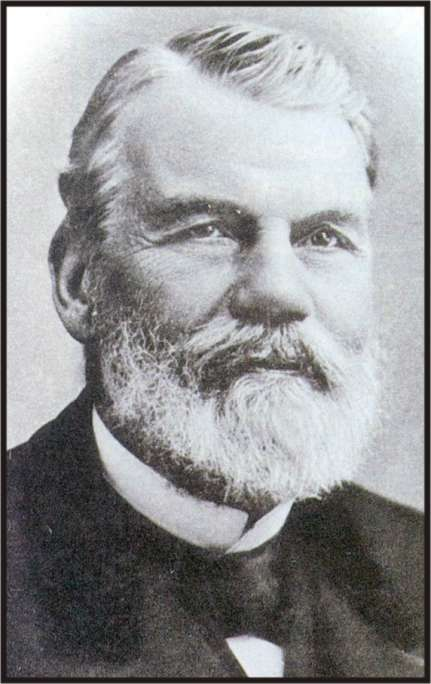
\includegraphics[width=\linewidth]{images/book3/raoult.jpg}
\end{minipage}\hfill
\begin{minipage}[t]{0.76\linewidth}\vspace{0pt}
فرانسوا ماري راوول (1830--1901)، أستاذ الكيمياء في غرونوبل، قاس خلال
ثمانينيات القرن التاسع عشر درجات تجمد مئات المحاليل ثم ضغوط بخارها،
ووجد أن الانخفاض، في المحاليل المخففة، يتعلق بعدد الجزيئات المذابة لا
بطبيعتها. وصارت قياساته طريقة لوزن الجزيئات، ودعمت النظرية الفتية للأيونات
في المحلول. (صورة: ملكية عامة، ويكيميديا كومنز.)
\end{minipage}
\end{history}

\section{الخلائط الحقيقية}

\begin{definition}[معامل النشاطية]\label{def:b2:chemical-potential:activity-coefficient}
في خليط حقيقي يُكتب \omterm{def:b2:chemical-potential:chemical-potential}{الجهد الكيميائي} $\mu_i = \mu_i^\circ +
RT\ln a_i$ مع $a_i = \gamma_i x_i$ (مرجع راوول) أو $a_i = \gamma_i
c_i/c^\circ$ (مرجع هنري). والعامل $\gamma_i$ هو \emph{معامل
النشاطية}\index{معامل النشاطية}: يقيس الابتعاد عن القانون المثالي،
ويؤول إلى 1 في النهاية التي يصح فيها القانون المرجعي.
\end{definition}

المعامل الأكبر من 1 يعني أن الجزيء أقل استقرارًا بجيرانه في الخليط منه في
الحالة المرجعية (انحراف موجب، كما في الشكل أعلاه)؛ والأصغر من 1 يعني أنه
أكثر استقرارًا. وحسب جيبس--دوهيم، يرتبط معاملا المكوّنين في خليط ثنائي:
ففي النموذج ذي الوسيط الواحد المستعمل في الشكل، $\ln\gamma_1 = Ax_2^2$
و$\ln\gamma_2 = Ax_1^2$، 
و$x_1\,\dd\ln\gamma_1 + x_2\,\dd\ln\gamma_2 = 0$ متحققة تطابقيًا.

أما الأيونات، التي تتآثر على مدى بعيد، فتظهر انحرافاتها عند تراكيز
صغيرة.

\begin{definition}[الشدة الأيونية]\label{def:b2:chemical-potential:ionic-strength}
\emph{الشدة الأيونية}\index{شدة أيونية} لمحلول هي $I =
\frac12\sum_i z_i^2\,b_i$، حيث $b_i$ مولالية الأيون $i$ (كمية المادة لكل
كيلوغرام من المذيب) و$z_i$ عدد شحنته.
\end{definition}

\begin{proposition}[قانون ديباي--هوكل الحدي]\label{prop:b2:chemical-potential:debye-huckel}
في محلول إلكتروليت مخفف جدًا، يخضع \omterm{def:b2:chemical-potential:activity-coefficient}{معامل النشاطية} المتوسط لأيونات ملح
للعلاقة $\log\gamma_\pm = -A\,|z_+z_-|\sqrt{I/b^\circ}$، مع $A
\approx 0.51$ للماء عند \qty{25}{\celsius} و$b^\circ =
\qty{1}{mol/kg}$.
\end{proposition}
\admitted

\begin{remark}[المجال والأصل]\label{rem:b2:chemical-potential:dh-range}
يأتي القانون من نموذج يحاط فيه كل أيون «بجوّ» منتشر من الشحنة المعاكسة،
يخفض جهده الكيميائي؛ والنموذج خارج نطاق هذا المقرر، لكن ثابته $A$ ينتج من
سماحية الماء وكثافته ومن درجة الحرارة. وهو دقيق تحت
نحو $I = \qty{0.01}{mol/kg}$. والجوّ الأيوني نفسه يبطئ الأيونات في
مجال كهربائي، ويفسر لماذا تنخفض الموصلية المولية لإلكتروليت قوي وفق
$\Lambda = \Lambda^\circ - K\sqrt c$ (قانون الجذر التربيعي لكولراوش)
بدل أن تبقى عند قيمتها الحدية: وهذا هو حد قانون كولراوش الذي لقيناه في
مجلد السنة الأولى.
% ledger: epsr:H2O, rho:water.298, const:e, const:eps0, const:kB, const:NA (A computed in figdata/bachelor-2/colligative.py)
\end{remark}

\begin{example}[ملح سنتيمولالي]\label{ex:b2:chemical-potential:dh}
من أجل كلوريد الصوديوم عند $b = \qty{0.010}{mol/kg}$، $I = \frac12(0.010 + 0.010)
= \qty{0.010}{mol/kg}$ و$\log\gamma_\pm = -0.51 \times 0.10$: $\gamma_\pm
= 0.89$. فمنذ جزء من مئة من المول لكل كيلوغرام، يؤدي أخذ التركيز مكان
النشاطية إلى خطأ قدره 11\,\%؛ ومن أجل ملح من نوع 2:2 مثل كبريتات
المغنيسيوم عند المولالية نفسها، $I = 0.040$ و$\gamma_\pm = 0.62$.
\end{example}

\section{الخواص التجميعية}

\begin{definition}[الخاصية التجميعية]\label{def:b2:chemical-potential:colligative}
\emph{الخاصية التجميعية}\index{خاصية تجميعية} لمحلول مخفف هي
خاصية تتعلق بكمية الجسيمات المذابة لكل كمية من المذيب لا بطبيعتها:
انخفاض ضغط البخار، وانخفاض درجة التجمد، وارتفاع درجة الغليان، \omterm{def:b2:chemical-potential:osmotic-pressure}{والضغط
الأسموزي}. وثابتا قانوني درجة التجمد ودرجة الغليان أدناه هما
\emph{الثابت الكريوسكوبي}\index{ثابت كريوسكوبي} $K_f$
و\emph{الثابت الإبوليوسكوبي}\index{ثابت إبوليوسكوبي} $K_b$
للمذيب.
\end{definition}

\begin{omfigure}
\begin{tikzpicture}[font=\small, >={Stealth}]
  \draw[->] (0,0) -- (8,0) node[right] {$T$};
  \draw[->] (0,0) -- (0,4.4) node[above] {\foreignlanguage{arabic}{$\mu$ للمذيب}};
  % slopes = -S_m: the liquid, more disordered, falls faster than the solid
  \draw[omDef, very thick] (0.4,3.0) -- (7.0,2.01) node[right] {صلب};
  \draw[omThm, very thick] (0.4,3.6) -- (7.6,0.72) node[right] {سائل نقي};
  \draw[omThm, very thick, dashed] (0.4,3.25) -- (7.6,0.37) node[right] {محلول};
  \fill (2.8,2.64) circle (1.5pt);
  \fill (1.4,2.85) circle (1.5pt);
  \draw[densely dotted] (2.8,2.64) -- (2.8,0) node[below] {$T_f^*$};
  \draw[densely dotted] (1.4,2.85) -- (1.4,0) node[below] {$T_f$};
  \draw[<->] (1.4,-0.75) -- (2.8,-0.75) node[midway, below] {$\Delta T_f$};
  \draw[<->, black!70] (5.0,1.76) -- (5.0,1.41);
  \draw[black!50] (5.0,1.58) -- (4.6,0.75) node[below, font=\scriptsize, black] {$RT\ln x_1$};
\end{tikzpicture}

{\small \omterm{def:b2:chemical-potential:chemical-potential}{الجهد الكيميائي} للمذيب بدلالة درجة الحرارة (رسم تخطيطي، عند ضغط
ثابت). الطور المستقر هو الطور ذو $\mu$ الأدنى. وإذابة مذاب تخفض خط السائل
بمقدار $RT\ln x_1 < 0$؛ فيلاقي خطَّ الجسم الصلب الآن عند درجة حرارة أدنى:
فيتجمد المحلول تحت درجة تجمد المذيب النقي.}
\end{omfigure}

\begin{theorem}[انخفاض درجة التجمد]\label{thm:b2:chemical-potential:cryoscopy}
يبدأ المحلول المخفف لمذاب لا يدخل في الجسم الصلب بالتجمد
عند $T_f = T_f^* - \Delta T_f$، مع
\[
  \Delta T_f = K_f\,b, \qquad K_f = \frac{R\,T_f^{*2}\,M_1}{\Delta_{\text{انصهار}}H_1} ,
\]
حيث $b$ المولالية الكلية للجسيمات المذابة و$M_1$ الكتلة المولية
للمذيب (بوحدة \unit{kg/mol}). ومن أجل تراكيز منتهية تكون العلاقة الدقيقة
لمحلول مثالي $\ln x_1 = -\frac{\Delta_{\text{انصهار}}H_1}{R}
\left(\frac{1}{T_f} - \frac{1}{T_f^*}\right)$.
\end{theorem}

\begin{proof}
عند نقطة التجمد يكون المذيب الصلب النقي والمذيب في المحلول في
توازن: $\mu_1^{\text{s}}(T) = \mu_1^{*\text{l}}(T) + RT\ln x_1$، ومنه
$\ln x_1 = -\Delta_{\text{انصهار}}G_1(T)/(RT)$، مع $\Delta_{\text{انصهار}}G_1 =
\mu_1^{*\text{l}} - \mu_1^{\text{s}}$، المنعدم عند $T_f^*$. وحسب جيبس--هلمهولتز،
$\dd(\Delta_{\text{انصهار}}G_1/T)/\dd T = -\Delta_{\text{انصهار}}H_1/T^2$؛
وبالمكاملة من $T_f^*$ إلى $T_f$ مع $\Delta_{\text{انصهار}}H_1$ ثابت نحصل على
العلاقة الدقيقة. ومن أجل محلول مخفف، $\ln x_1 = \ln(1 - x_2) \approx
-x_2$ و$\frac1{T_f} - \frac1{T_f^*} \approx -\Delta T_f/T_f^{*2}$، ومنه
$x_2 = \Delta_{\text{انصهار}}H_1\Delta T_f/(RT_f^{*2})$؛ وأخيرًا $x_2 \approx
n_2/n_1 = b\,M_1$.
\end{proof}

\begin{proposition}[ارتفاع درجة الغليان]\label{prop:b2:chemical-potential:ebullioscopy}
يغلي المحلول المخفف لمذاب غير متطاير عند $T_b^* + \Delta T_b$ مع
$\Delta T_b = K_b\,b$، $K_b = RT_b^{*2}M_1/\Delta_{\text{تبخر}}H_1$.
\end{proposition}

\begin{proof}
البرهان نفسه، مع البخار مكان الجسم الصلب: $\mu_1^{*\text{l}} +
RT\ln x_1 = \mu_1^{\text{v}}$؛ فينخفض خط المذيب، ويلاقي الآن خط
البخار عند درجة حرارة أعلى.
\end{proof}

\begin{example}[الماء]\label{ex:b2:chemical-potential:water-constants}
مع $\Delta_{\text{انصهار}}H = \qty{333.4}{J/g} = \qty{6.007}{kJ/mol}$ عند
\qty{273.15}{K}: $K_f = 8.314 \times 273.15^2 \times 0.018015/6007 =
\qty{1.86}{K.kg/mol}$. ومع $\Delta_{\text{تبخر}}H = \qty{40.65}{kJ/mol}$ عند
\qty{373.12}{K}: $K_b = \qty{0.513}{K.kg/mol}$. وماء البحر، \qty{35}{g} من الملح
لكل كيلوغرام، محسوبًا كلوريدَ صوديوم (جسيمان لكل صيغة):
$b = 2 \times 35/58.44/0.965 = \qty{1.24}{mol/kg}$، فيتنبأ القانون المخفف
بالقيمة \qty{-2.3}{\celsius}، وهي مبالغ فيها: ففي هذا التركيز تكون
الأيونات بعيدة عن المثالية، وملح البحر ليس كله كلوريد صوديوم.
% ledger: dfus:H2O, tfus:H2O, dvap:H2O.nbp, tb:H2O.atm, sea:salinity (computed in figdata/bachelor-2/colligative.py)
\end{example}

\begin{definition}[الغشاء نصف النفوذ، الضغط الأسموزي]\label{def:b2:chemical-potential:osmotic-pressure}
\emph{الغشاء نصف النفوذ}\index{غشاء نصف نفوذ} يسمح بمرور
المذيب لا المذاب. وحين يفصل محلولًا عن المذيب النقي، يتدفق المذيب نحو
المحلول؛ و\emph{الضغط الأسموزي}\index{ضغط أسموزي} $\Pi$ هو فائض الضغط الذي يجب
تطبيقه على المحلول لإيقاف هذا التدفق.
\end{definition}

\begin{theorem}[قانون فانت هوف الأسموزي]\label{thm:b2:chemical-potential:osmosis}
من أجل محلول مخفف، $\Pi = c\,RT$، حيث $c$ التركيز الكلي للجسيمات
المذابة.
\end{theorem}

\begin{proof}
عند التوازن يكون للمذيب \omterm{def:b2:chemical-potential:chemical-potential}{الجهد الكيميائي} نفسه على الجانبين:
$\mu_1^*(T, p) = \mu_1^*(T, p + \Pi) + RT\ln x_1$. ولأن $(\partial\mu_1^*/
\partial p)_T = V_{m,1}$، الثابت تقريبًا لسائل، فإن $\mu_1^*(T, p + \Pi) -
\mu_1^*(T, p) = \Pi V_{m,1}$، ومنه $\Pi V_{m,1} = -RT\ln x_1 \approx RT x_2
\approx RT\,n_2/n_1$. ومع $n_1V_{m,1} \approx V$ (محلول مخفف)، $\Pi = n_2RT/V$.
\end{proof}

\begin{omfigure}
\begin{tikzpicture}[font=\small, >={Stealth}]
  \begin{scope}
    \clip (-0.85,2.8) -- (-0.85,0.85) arc[start angle=180, end angle=360,
      radius=0.85] -- (0.85,2.8) -- (0.55,2.8) -- (0.55,0.85)
      arc[start angle=0, end angle=-180, radius=0.55] -- (-0.55,2.8) -- cycle;
    \fill[omDef!18] (-1,0) rectangle (0,1.6);
    \fill[omThm!22] (0,0) rectangle (1,2.3);
  \end{scope}
  \pic at (0,0) {utube={0}{white}};
  \draw[very thick, dashed] (0,-0.05) -- (0,0.36);
  \node[left] at (-1.0,1.2) {ماء نقي};
  \node[right] at (1.0,0.9) {محلول};
  \draw[densely dotted] (-0.55,1.6) -- (1.55,1.6);
  \draw[densely dotted] (0.85,2.3) -- (1.55,2.3);
  \draw[<->, thick] (1.45,1.6) -- (1.45,2.3) node[midway, right] {\foreignlanguage{arabic}{$h$، مع $\Pi = \rho g h$}};
  \draw (0,0.12) -- (0.6,-0.5) node[below right] {غشاء نصف نفوذ};
  \draw[->, omDef, thick] (-0.75,0.4) to[bend right=30] (-0.25,0.12);
\end{tikzpicture}

{\small \omterm{def:b2:chemical-potential:osmotic-pressure}{الضغط الأسموزي} في أنبوب على شكل U. يعبر الماء الغشاء نحو المحلول
حتى يساوي الضغط الهيدروستاتيكي الإضافي للعمود الأعلى الضغطَ الأسموزي؛
وعندئذ يتساوى \omterm{def:b2:chemical-potential:chemical-potential}{الجهد الكيميائي} للماء على الجانبين.}
\end{omfigure}

\begin{method}[الكتلة المولية بخاصية تجميعية]\label{met:b2:chemical-potential:molar-mass}
\begin{enumerate}
  \item أذب كتلة معلومة $m_2$ من المادة في كتلة معلومة $m_1$
        من المذيب (أو في حجم معلوم $V$ من المحلول).
  \item قِس $\Delta T_f$ (أو $\Delta T_b$، أو $\Pi$).
  \item استنتج المولالية $b = \Delta T_f/K_f$ (أو $c = \Pi/RT$)، ثم $n_2 =
        b\,m_1$ (أو $cV$) و$M_2 = m_2/n_2$؛ واقسم على عدد
        الجسيمات لكل صيغة إن كانت المادة تتفكك.
\end{enumerate}
يلائم قياس \omterm{def:b2:chemical-potential:osmotic-pressure}{الضغط الأسموزي} الجزيئات الكبيرة (البروتينات، البوليمرات): فبضعة
غرامات في اللتر من بروتين كتلته المولية \qty{60}{kg/mol} تعطي بضع مئات من
الباسكالات، أي ملّيمترات من الماء، لكنها لا تغير درجة التجمد إلا ببضعة أجزاء
من الألف من الكلفن.
\end{method}

\section{تمارين}

\begin{exercise}[$\star$]\label{exo:b2:chemical-potential:1}
استعمل إنشاء المماس على شكل الحجم المولي (خليط نموذجي)
عند $x_2 = 0.4$ لقراءة $\bar V_1$ و$\bar V_2$، وتحقق من أن
$x_1\bar V_1 + x_2\bar V_2$ هو الحجم المولي للخليط.
\end{exercise}

\begin{exercise}[$\star$]\label{exo:b2:chemical-potential:2}
عند \qty{25}{\celsius} يكون ضغط بخار الماء \qty{3.17}{kPa}.
احسب، \omterm{thm:b2:chemical-potential:raoult}{بقانون راوول}، ضغط البخار فوق محلول فيه
\qty{1.00}{mol} من السكروز (غير متطاير) في \qty{1.00}{kg} من الماء.
% ledger: pvap:H2O.298
\end{exercise}

\begin{exercise}[$\star$]\label{exo:b2:chemical-potential:3}
احسب تركيز ثنائي الأكسجين المذاب في ماء في توازن مع
هواء عند \qty{1.013}{bar} و\qty{25}{\celsius} ($H(\ce{O2}) =
\qty{1.3e-5}{mol/(m^3.Pa)}$، و\qty{20.95}{\percent} من ثنائي الأكسجين)، بوحدة
\unit{mol/L} وبوحدة \unit{mg/L}.
% ledger: henry:O2, air:O2
\end{exercise}

\begin{exercise}[$\star$]\label{exo:b2:chemical-potential:4}
من أجل \ce{N2(g) + 3H2(g) <=> 2NH3(g)} عند \qty{298}{K}، $\Delta_r G^\circ =
\qty{-32.8}{kJ/mol}$. احسب $\Delta_r G$ في خليط فيه
$p(\ce{N2}) = \qty{1.0}{bar}$، و$p(\ce{H2}) = \qty{0.010}{bar}$،
و$p(\ce{NH3}) = \qty{1.0}{bar}$، وبيّن في أي اتجاه يجري التفاعل.
\end{exercise}

\begin{exercise}[$\star\star$]\label{exo:b2:chemical-potential:5}
في خليط ثنائي، يتغير \omterm{def:b2:chemical-potential:partial-molar}{الحجم المولي الجزئي} للمكوّن 1 بمقدار
$\dd\bar V_1 = \qty{-0.30}{mL/mol}$ حين ينتقل $x_2$ من 0.30 إلى 0.31. أوجد
$\dd\bar V_2$ مستعملًا علاقة جيبس--دوهيم.
\end{exercise}

\begin{exercise}[$\star\star$]\label{exo:b2:chemical-potential:6}
يحوي المحلول الملحي الفيزيولوجي \qty{9.0}{g} من كلوريد الصوديوم في اللتر.
احسب ضغطه الأسموزي عند \qty{37}{\celsius}، مع عدّ الملح تام
التفكك، وفسّر لماذا تحافظ كريات الدم الحمراء على شكلها فيه لكنها تنتفخ
وتنفجر في الماء النقي.
\end{exercise}

\begin{exercise}[$\star\star$]\label{exo:b2:chemical-potential:7}
لمحلول فيه \qty{2.00}{g} من بروتين في \qty{100.0}{mL} من الماء \omterm{def:b2:chemical-potential:osmotic-pressure}{ضغط
أسموزي} قدره \qty{0.825}{kPa} عند \qty{25}{\celsius}. احسب الكتلة المولية
للبروتين، وانخفاض درجة تجمد هذا المحلول.
\end{exercise}

\begin{exercise}[$\star\star$]\label{exo:b2:chemical-potential:8}
احسب \omterm{def:b2:chemical-potential:ionic-strength}{الشدة الأيونية} \omterm{def:b2:chemical-potential:activity-coefficient}{ومعاملات النشاطية} المتوسطة (القانون الحدي)
لكل من: (أ) كلوريد الصوديوم بمولالية \qty{1.0e-3}{mol/kg}؛ (ب) كلوريد
الكالسيوم بمولالية \qty{1.0e-3}{mol/kg}؛ (ج) كبريتات المغنيسيوم بمولالية \qty{1.0e-3}{mol/kg}.
\end{exercise}

\begin{exercise}[$\star\star$]\label{exo:b2:chemical-potential:9}
يتجمد محلول فيه \qty{1.50}{g} من مركب مجهول غير متطاير ولا يتفكك
في \qty{50.0}{g} من الماء عند \qty{-0.310}{\celsius}. احسب
كتلته المولية.
\end{exercise}

\begin{exercise}[$\star\star\star$]\label{exo:b2:chemical-potential:10}
بيّن أنه في النموذج ذي الوسيط الواحد $\ln\gamma_1 = Ax_2^2$، $\ln\gamma_2 =
Ax_1^2$، تتحقق علاقة جيبس--دوهيم، وأن \omterm{prop:b2:chemical-potential:henry}{ثابت هنري} للمكوّن 1 هو
$k_{H,1} = p_1^*\mathrm e^A$. ومن أجل $A = 1.1$، بأي عامل يزيد ميل هنري
على ميل راوول؟
\end{exercise}

\begin{exercise}[$\star\star\star$]\label{exo:b2:chemical-potential:11}
فسّر لماذا يحتاج قانون تجميعي (أ) إلى مذاب غير متطاير من أجل ارتفاع
درجة الغليان، و(ب) إلى مذاب لا يدخل في الجسم الصلب من أجل انخفاض درجة
التجمد. ماذا يحدث لدرجة تجمد مذيب يكوّن مذابه معه محلولًا صلبًا مثاليًا
بالنسبة نفسها التي في السائل؟
\end{exercise}

\begin{exercise}[$\star\star\star$]\label{exo:b2:chemical-potential:12}
يقرأ محرار حتى \qty{0.01}{K}. احسب أصغر مولالية لمذاب لا يتفكك
يمكن كشفها في الماء بقياس انخفاض درجة التجمد وبقياس ارتفاع درجة الغليان،
\omterm{def:b2:chemical-potential:osmotic-pressure}{والضغط الأسموزي} الموافق عند \qty{25}{\celsius}.
أي الطرائق أشد حساسية، ولماذا تُستعمل مقاييس \omterm{def:b2:chemical-potential:osmotic-pressure}{الضغط الأسموزي} للبوليمرات؟
\end{exercise}

\section{مسألة: المبرّد في الشتاء}

\begin{problem}[{مسألة نهاية الأسبوع --- \omterm{def:b2:chemical-potential:ideal-mixture}{خليط مثالي} من الماء
والإيثان-1,2-ديول، والقانون الكريوسكوبي وثابته، وتجمد سائل تبريد، وكم
من الديول يُبقي المحرك سائلًا عند \qty{-20}{\celsius}}]
\label{pb:b2:chemical-potential:1}
سائل تبريد المحرك خليط من الماء والإيثان-1,2-ديول
(\ce{HOCH2CH2OH}، $M = \qty{62.07}{g/mol}$، درجة غليانه \qty{197}{\celsius}،
غير متطاير هنا). الماء: $M = \qty{18.015}{g/mol}$، ودرجة تجمده
\qty{273.15}{K}، وأنتالبي انصهاره \qty{333.4}{J/g}، ودرجة غليانه
\qty{373.12}{K} تحت \qty{1.013}{bar}، وأنتالبي تبخره
\qty{40.65}{kJ/mol}، وضغط بخاره \qty{3.17}{kPa} عند \qty{25}{\celsius}.
ويُعدّ الخليط مثاليًا.
% ledger: tb:glycol, dfus:H2O, tfus:H2O, tb:H2O.atm, dvap:H2O.nbp, pvap:H2O.298

\medskip
\noindent\textbf{الجزء الأول --- الخليط.}
\begin{enumerate}
  \item اكتب \omterm{def:b2:chemical-potential:chemical-potential}{الجهد الكيميائي} للماء في \omterm{def:b2:chemical-potential:ideal-mixture}{خليط مثالي}.
  \item يحوي سائل تبريد \qty{30}{\percent} من الديول كتلةً. احسب
        كميتي مادة الديول والماء في \qty{100}{g}، والكسر المولي
        للماء.
  \item احسب ضغط بخار الماء فوق سائل التبريد هذا عند
        \qty{25}{\celsius}.
  \item احسب مولالية الديول.
  \item لماذا يُهمل ضغط بخار الديول نفسه؟
\end{enumerate}

\medskip
\noindent\textbf{الجزء الثاني --- القانون الكريوسكوبي.}
\begin{enumerate}[resume]
  \item اكتب تساوي الجهود الكيميائية عند نقطة تجمد سائل التبريد،
        والجسم الصلب جليد نقي.
  \item مستعملًا علاقة جيبس--هلمهولتز، استنتج $\ln x_1 =
        -\frac{\Delta_{\text{انصهار}}H}{R}\left(\frac1{T_f} - \frac1{T_f^*}\right)$.
  \item اجعلها خطية من أجل محلول مخفف واستنتج $\Delta T_f = K_f b$.
  \item احسب أنتالبي الانصهار المولي للماء والثابت $K_f$.
  \item ما الفرض الذي وضعته المكاملة على أنتالبي
        الانصهار؟
\end{enumerate}

\medskip
\noindent\textbf{الجزء الثالث --- التجمد.}
\begin{enumerate}[resume]
  \item احسب درجة تجمد سائل التبريد ذي \qty{30}{\percent} بالقانون
        المخفف.
  \item احسبها بالعلاقة المثالية الدقيقة.
  \item أي النتيجتين أجدر بالثقة، ولماذا لا تعدو كلتاهما تقديرًا لسائل
        تبريد حقيقي؟
  \item ماذا يتبلور عند نقطة التجمد؟
  \item بمتابعة التبريد يغتني السائل المتبقي بالديول. فسّر
        لماذا يستمر تكوّن الجليد عند درجات حرارة تزداد انخفاضًا.
\end{enumerate}

\medskip
\noindent\textbf{الجزء الرابع --- الغليان، وهدف الشتاء.}
\begin{enumerate}[resume]
  \item احسب $K_b$ للماء.
  \item احسب ارتفاع درجة غليان سائل التبريد ذي \qty{30}{\percent}
        عند \qty{1.013}{bar}.
  \item المبرّد مضغوط حتى \qty{2.0}{bar}. مستعملًا علاقة
        كلاوزيوس--كلابيرون المعروفة من الفيزياء مع أنتالبي التبخر
        أعلاه، قدّر درجة غليان الماء النقي عند
        \qty{2.0}{bar}.
  \item أيهما أهم في الصيف، الغطاء المضغوط أم الديول؟
  \item من أجل سائل تبريد يبقى سائلًا حتى \qty{-20}{\celsius}، احسب الكسر
        المولي للماء الذي تتطلبه العلاقة المثالية الدقيقة.
  \item حوّله إلى كسر كتلي للديول.
  \item احسب الكسر الكتلي الذي كان سيعطيه القانون المخفف،
        وفسّر الفرق.
  \item اذكر الكسر الكتلي للديول الذي يُبقي سائل التبريد سائلًا حتى
        \qty{-20}{\celsius} في نموذج \omterm{def:b2:chemical-potential:ideal-mixture}{الخليط المثالي}.
\end{enumerate}
\end{problem}
